\documentclass[11pt]{article}

\usepackage[T1]{fontenc}
\usepackage[utf8]{inputenc}
\usepackage[margin=0.82in]{geometry}
\usepackage{amsmath,amssymb}
\usepackage{array,booktabs,longtable,tabularx}
\usepackage{enumitem}
\usepackage{graphicx}
\usepackage{microtype}
\usepackage{seqsplit}
\usepackage{xcolor}
\usepackage[hidelinks]{hyperref}

\setlist{nosep,leftmargin=*}
\setlength{\emergencystretch}{2em}
\urlstyle{tt}

\definecolor{passgreen}{RGB}{20,120,70}
\definecolor{failred}{RGB}{170,35,35}
\definecolor{pendingblue}{RGB}{30,80,155}
\definecolor{warningamber}{RGB}{160,95,0}
\newcommand{\pass}{\textcolor{passgreen}{\textbf{PASS}}}
\newcommand{\fail}{\textcolor{failred}{\textbf{FAIL}}}
\newcommand{\pending}{\textcolor{pendingblue}{\textbf{PENDING}}}
\newcommand{\risk}{\textcolor{warningamber}{\textbf{RISK}}}
\newcommand{\code}[1]{\texttt{#1}}
\newcommand{\hash}[1]{{\ttfamily\footnotesize\seqsplit{#1}}}
\newcommand{\plannedresult}[1]{%
  \begin{center}
  \fbox{\parbox{0.92\linewidth}{\textcolor{pendingblue}{\textbf{Pending result.}} #1}}
  \end{center}
}
\newcommand{\plannedfigure}[1]{%
  \begin{center}
  \fbox{\parbox[c][1.05in][c]{0.88\linewidth}{\centering
  \textcolor{pendingblue}{\textbf{Planned figure:}} #1}}
  \end{center}
}

\title{Agent-Population Scaling and Decentralized Team Recruitment in Alem\\
\large Combined E0--E3 Methods, Results, and Preregistered Evaluation Report}
\author{AlemDICE Research Engineering Report}
\date{23 July 2026}

\begin{document}
\maketitle

\begin{abstract}
This report consolidates a staged investigation of physical-agent scaling,
decentralized team recruitment, and team-scoped communication in Alem.
The completed evidence includes two provider-free engineering studies, a
15-episode hosted Source population screen, and a bounded hosted six-agent
recruitment mechanism screen.
E0 exercised the canonical evaluator at
$N\in\{1,2,3,4,6\}$ for two seeds and ten ticks and passed every structural,
accounting, replay, and renderer gate.  E0.1 requested 200 ticks with the same
scripted \code{Noop} policy.  All structural gates again passed, but only seven
of ten episodes reached the requested horizon; three ended normally after all
agents died.  E0.1 is therefore a structural \pass{} and a literal
full-horizon \fail{}.  Neither study measures useful behavior.

E1 completed three paired 200-requested-tick seeds at each population.  Source
Total score and return rose through three agents, were similar at four, and
fell at six while mean delivered bytes, tokens, and tick wall time continued
to rise.  The six-agent arm is a Source-as-implemented stress result rather
than a clean population effect: hard mining and construction can require all
six agents even though collision-free cardinal interaction geometry permits at
most four simultaneous targeters.

E2b v2 and v3 remain poisoned, non-promotable diagnostics.  The prospectively
frozen Open-only v4 confirmation completed all 12 cells, achieved full reward
and oracle-allocation coverage in 12/12, and formed 15/15 true-feasible locks
without transport error, incomplete response, or output truncation in 293
calls.  Ten of 12 whole allocations exactly matched the true oracle; mean
utility regret was 0.005660 and mean raw-cost delta was $+4.9167$.  These
results promote only Open Volunteer with truth-free joint exact allocation to
a bounded, feasibility-controlled E3 Alem transfer.  E3 remains prospective,
so embodied team efficacy, intrinsic population scalability, context
management, and long-horizon role alignment are not yet established.
\end{abstract}

\section{Program status and claim boundary}

\begin{table}[ht]
\centering
\small
\begin{tabularx}{\textwidth}{@{}l l X@{}}
\toprule
Stage & Status & Current evidence or blocker\\
\midrule
E0: 10-tick compatibility & \pass &
Ten provider-free episodes completed; all structural gates and five renderer
smokes passed.\\
E0.1: 200-tick extension & \pass{} structural / \fail{} horizon &
Ten complete artifact sets; 7/10 episodes reached tick 200; three terminated
naturally after all-agent death.\\
E1: Source population curve & \pass{} complete / \risk{} $N=6$ confound &
All 15 cells completed and reconciled.  Performance peaked at $N=3$--4 and
declined at $N=6$ as cost rose, but six-agent hard-sync tasks can be
geometrically impossible.\\
E2: RecruitmentArena-6 & \pass{} provider-free / \fail{} v2--v3 / \pass{} v4 &
TFP1, arena, policies, selectors, oracle, and the staged E2b harness are
implemented.  E2d2 promoted joint exact allocation.  E2b v2 failed after 72
hosted calls; the v3 canary failed after 40.  Open-only v4 passed 12/12
episodes and 15/15 true-feasible locks in 293 calls.\\
E3: Alem recruitment & \risk{} protocol frozen / not runnable &
The narrow Open/joint-exact transfer is specified, but opt-in routing, task
binding, feasibility control, and provider-free E3a gates remain unimplemented.\\
\bottomrule
\end{tabularx}
\caption{Status at the report date.  ``Pending'' denotes an unobserved study,
not a null or negative result.}
\label{tab:status}
\end{table}

The program asks three ordered questions:

\begin{enumerate}
  \item \textbf{Population scaling:} How does the unchanged Source language
  agent behave as the number of physical agents changes?
  \item \textbf{Formation mechanism:} Can six embodied agents form useful,
  task-bound teams using bounded decentralized recruitment records?
  \item \textbf{Environment transfer:} Does a promoted recruitment mechanism
  retain useful performance in Alem when ordinary conversation is restricted
  to current teammates?
\end{enumerate}

Each stage removes a distinct ambiguity.  E0 separates infrastructure from
model behavior.  E1 measures population behavior before routing is altered.
E2 separates recruitment from the full game.  E3 tests whether the mechanism
survives the navigation, survival, and action constraints of Alem.  A failure
at an earlier gate blocks downstream efficacy claims.

The completed sequence may support claims about population scaling,
decentralized team formation, and team-scoped communication.  It does not by
itself establish strict information isolation, robustness to adversarial or
crashed agents, learned communication, long-horizon role alignment, or
populations above six.

\section{Shared experimental conventions}

\subsection{Behavioral model and unchanged Source condition}

All paid behavioral stages use homogeneous GPT-5.4 nano action agents with
reasoning effort \code{high}.  The Source arm retains:

\begin{itemize}
  \item the \code{robust\_all} agent;
  \item the \code{specific\_collaborative} prompt;
  \item normal reasoning and scratchpad memory;
  \item the existing action parser and legal-action affordances;
  \item one model call per physical agent per environment tick; and
  \item ordinary one-tick-delayed peer broadcast.
\end{itemize}

No bodyless leader, extra planner, or additional planning call is part of this
program.  Agent calls within a tick run concurrently.  Behavioral arms use one
episode worker unless a separate provider-load experiment is preregistered.

\subsection{Paired designs and terminal episodes}

Comparisons use identical environment seeds across arms.  A natural all-agent
death is a valid terminal outcome, not an API failure.  Every report must state
both the requested horizon and actual executed ticks.  Cost denominators include
actual physical agent-ticks so early death cannot appear to improve efficiency.

\subsection{Primary outcomes}

The three co-primary Alem outcomes are:

\begin{enumerate}
  \item paper Total achievement percentage;
  \item mean per-agent episode return; and
  \item raw unique team achievements.
\end{enumerate}

Supporting outcomes include Base and Coordination achievement percentages,
deaths, alive-agent steps, action parse rate, task attempts and successes,
messages, emitted bytes, delivered bytes, tokens, model latency, and complete
tick wall time.  Formation studies additionally report normalized task reward,
oracle regret, feasible-team rate, formation latency, churn, roster agreement,
and truthful-report calibration.

\section{E0: short variable-agent compatibility gate}

\subsection{Method}

E0 crossed $N\in\{1,2,3,4,6\}$ with seeds 13000 and 13001 for ten ticks in
\code{alem/default}, Easy coordination difficulty, and baseline communication.
Exactly one indexed client configuration existed per physical agent, but a
deterministic test actor replaced inference.  Every actor selected
\code{Noop} and emitted
\[
\code{E0|AGENT=}\,i\,\code{|TICK=}\,t\,\code{|STATE=ACTIVE}.
\]
The normal evaluator still performed reset, stepping, action canonicalization,
one-tick routing, trajectory and state serialization, debug output, terminal
accounting, and attempt-ledger writing.

The gate checked:

\begin{itemize}
  \item client and agent cardinality and every trajectory agent axis;
  \item Warrior, Forager, Miner specialization cycling;
  \item every ordered \code{Give to Agent $j$} mapping;
  \item action parse rate equal to one;
  \item zero model calls, provider requests, and transport errors;
  \item exact baseline accounting,
  $M_{\mathrm{emit}}=NT$ and
  $M_{\mathrm{deliver}}=N(N-1)T$;
  \item complete canonical artifacts and ten state snapshots per episode; and
  \item equality of stable reset and saved-state projection hashes.
\end{itemize}

One seed-13000 state at every population was also encoded as a 768-by-832 H.264
full-world renderer smoke artifact and validated with \code{ffprobe}.

\subsection{Measured result}

\begin{table}[ht]
\centering
\small
\resizebox{\textwidth}{!}{%
\begin{tabular}{@{}rrrrrrrrrc@{}}
\toprule
$N$ & Episodes & Ticks & Observation dim. & Actions & Give maps &
Emitted & Delivered & Delivery bytes & Result\\
\midrule
1 & 2 & 20 & 9,476  & 55 & 0  & 20  & 0   & 0      & \pass\\
2 & 2 & 20 & 9,597  & 55 & 2  & 40  & 40  & 1,200  & \pass\\
3 & 2 & 20 & 9,718  & 56 & 6  & 60  & 120 & 3,600  & \pass\\
4 & 2 & 20 & 9,839  & 57 & 12 & 80  & 240 & 7,200  & \pass\\
6 & 2 & 20 & 10,081 & 59 & 30 & 120 & 600 & 18,000 & \pass\\
\bottomrule
\end{tabular}}
\caption{E0 measured results.  Give mappings count ordered
giver--recipient pairs, hence $N(N-1)$.}
\label{tab:e0}
\end{table}

Across ten episodes, E0 executed 100 environment ticks and 320 scripted
agent-ticks, emitted 320 messages, delivered 1,000 copies totaling 30,000
bytes, and saved 100 states.  All structural and renderer gates passed.
Observation length increased by 121 values for each added teammate.  Baseline
delivery fan-out grew quadratically.  These are interface and accounting
facts, not behavioral benefits.

\subsection{E0 decision}

E0 removed the short-run engineering blocker for the supported
$N=1,2,3,4$ screen and for the separately labeled $N=6$ extension.  It did not
test task performance, useful coordination, model reasoning, provider
concurrency, recruitment, or role coherence.

\section{E0.1: 200-requested-tick compatibility extension}

\subsection{Method and decision rule}

E0.1 repeated the same populations, seeds, scripted actor, Easy environment,
and baseline topology with 200 requested ticks.  It added monotonic timing for
the full episode, the complete evaluator tick, the slowest tick, and the
concurrent scripted-worker phase.

Two decisions were fixed:

\begin{description}[style=nextline,leftmargin=1.5em]
  \item[Structural gate.]
  Natural termination is allowed, but every episode must produce complete
  artifacts and pass all shape, action, role, communication, replay, and
  provider-accounting checks.
  \item[Strict horizon gate.]
  Every episode must execute all 200 requested ticks in addition to passing the
  structural gate.
\end{description}

\subsection{Measured gate outcomes}

All ten artifact sets were complete and every structural check passed.  Seven
episodes reached tick 200.  Three ended normally when all agents died from mob
combat:

\begin{itemize}
  \item $N=1$, seed 13000: 114/200 ticks and one death;
  \item $N=4$, seed 13001: 182/200 ticks and four deaths; and
  \item $N=6$, seed 13001: 192/200 ticks and six deaths.
\end{itemize}

Consequently, E0.1 is a structural \pass{} and a strict-horizon \fail{}.  The
failure is retained rather than being reclassified after observing that it was
a clean environment termination.

\begin{table}[ht]
\centering
\scriptsize
\resizebox{\textwidth}{!}{%
\begin{tabular}{@{}rrrrrrrrcc@{}}
\toprule
$N$ & Actual/requested ticks & Mean return & Full horizon & Alive-step \% &
Deaths/slots & Mean tick (s) & Mean excl.\ max (s) & Structural & Horizon\\
\midrule
1 & 314/400 & -0.4500 & 1/2 & N/A    & 1/2  & 0.151301 & 0.076475 & \pass & \fail\\
2 & 400/400 & -0.5250 & 2/2 & 95.88  & 1/4  & 0.175483 & 0.124436 & \pass & \pass\\
3 & 400/400 & -0.0333 & 2/2 & 100.00 & 0/6  & 0.235863 & 0.179381 & \pass & \pass\\
4 & 382/400 & -0.8625 & 1/2 & 78.73  & 7/8  & 0.296600 & 0.236695 & \pass & \fail\\
6 & 392/400 & -0.6833 & 1/2 & 86.48  & 8/12 & 0.437702 & 0.379037 & \pass & \fail\\
\bottomrule
\end{tabular}}
\caption{E0.1 structural, terminal, descriptive return, and timing results.
Return is mean cumulative reward per physical agent.  ``Mean excl.\ max''
removes exactly one slowest tick from each episode and is descriptive rather
than a separately timed warm benchmark.}
\label{tab:e01}
\end{table}

The matrix executed 1,888/2,000 requested environment ticks and
6,194/6,400 requested scripted agent-ticks.  It recorded 6,194 emitted
messages, 19,544 delivered copies, 614,408 delivered bytes, 1,888 saved states,
and zero model calls, provider requests, or transport errors.  The summed
episode wall time was 498.207821 seconds; end-to-end elapsed time was
659.272638 seconds.  The step-weighted complete-tick mean was 0.263203 seconds,
and the scripted-worker phase totaled only 0.326201 seconds.

Every achievement, normalized task-reward, player-progression, and monster-kill
field was zero.  Multi-agent coordination and item-give attempt counts were
also zero.  The nonpositive return therefore reflects net health change under
\code{Noop}, not task accomplishment.  The two-seed returns and mortality
patterns cannot rank populations.

\subsection{E0.1 decision}

E0.1 strengthens the engineering evidence that the evaluator and artifact path
support variable populations over substantially longer runs.  It does not show
that an inactive policy survives to a fixed horizon.  Behavioral experiments
must treat all-agent death as an outcome and normalize exposure by actual
agent-ticks.

\section{E1 completed screen: Source performance versus population}

\subsection{Questions and hypotheses}

E1 asks how the unchanged Source condition behaves as physical population
changes.  It is intentionally descriptive because changing $N$ also changes
spawn geometry, role balance, mob slots, prompt size, teammate observations,
communication fan-out, and some coordination requirements.

\begin{description}[style=nextline,leftmargin=1.5em]
  \item[H1a: behavioral scaling.]
  Useful task performance will vary detectably with population, but no
  monotonic direction is assumed in advance.
  \item[H1b: communication scaling.]
  Under full broadcast, delivered message copies and bytes will increase
  approximately with $N(N-1)$ conditional on emission rate.
  \item[H1c: efficiency tradeoff.]
  Any performance gain at larger $N$ may be offset by greater token,
  communication, and complete-tick cost.
\end{description}

\subsection{Fixed configuration and funnel}

The behavioral model is GPT-5.4 nano at high reasoning with
\code{robust\_all}, \code{specific\_collaborative}, scratchpad, action parser,
and free peer broadcast.  Debriefs and bulk image generation are disabled.
Agents within a tick are called concurrently; episodes use one worker.

The executable profile is \code{source\_scaling\_200}.  It declares six client
slots but the launcher overrides only physical population size; surplus slots
are never instantiated as agents.  Provider reasoning is controlled by
\code{reasoning\_effort=high}; the local-model \code{agent.reasoning} switch
remains unset.  Population-and-agent-specific prompt-cache keys use one stable
traffic shard, so an interrupted resume returns to the same route rather than
reassigning a remaining seed to another seed's shard.

Before any episode call, a dedicated cache route makes one bounded
GPT-5.4-nano-high compatibility request and requires an exact parse of
\code{<action>Noop</action>}.  Its source commit, dependency lock, resolved
configuration hash, response ID, provider status, usage, latency, transport
attempts, and effective cache key are written durably.  The episode campaign
then has a nominal ceiling of 6,000 logical calls for E1a and 3,600 for E1b.
Hard campaign ceilings are 12,001 successful logical responses including the
preflight and 15,000 observed provider attempts.  An exclusive run lock,
atomic manifests, exact cell-identity checks, append-only attempt ledgers, and
child-process cleanup protect paid resume.

The frozen provider wrapper permits at most five retryable transport failures
before a logical call is exhausted.  A recovered transport retry is therefore
not treated as an episode failure.  Acceptance instead requires the exact
identity
\[
  \text{provider attempts}
  =
  \text{completed logical responses}
  +
  \text{transport errors}
\]
globally and for every physical worker, typed error counts that reconcile to
the global count, one unique final completed response per decision, complete
model/token evidence, zero incomplete responses, and exact agreement with the
append-only attempt ledger.  New versioned artifacts retain this evidence for
each logical call.  The frozen legacy artifacts retain final-response usage
per call and retry totals per worker; when only one worker has a retry, its
typed error ownership is exact by elimination and is labeled as legacy
aggregate reconstruction.  Unaccounted attempts, errors distributed across
workers without type attribution, exhausted calls, and campaign-cap overruns
remain disqualifying.

The completed campaign contains all 15 preregistered population--seed cells.
Episode artifacts contain 9,573 completed logical responses and 9,574 provider
attempts.  The only retry was one recovered \code{APIConnectionError} on worker
2 at $N=4$, seed 13101; no logical call was lost and no response was
incomplete.  Including the clean preflight, usage was 9,574 of 12,001 logical
responses and 9,575 of 15,000 provider attempts.  Fourteen episodes reached
the 200-tick truncation cap; $N=3$, seed 13102 terminated naturally at tick
191, exactly accounting for 27 fewer agent decisions than the nominal 9,600.

Each terminal artifact includes the
\code{alem-dice-performance-v1} block.  Base, Coordination, and Total are
reward-weighted paper scores on a 0--100 scale.  Unique team achievement counts
are binary first-unlocks by achievement type; summed per-agent counts may count
the same type once for each attaining agent.  They are not repeated world-event
counts.  Separate cumulative counters retain coordination attempts, resolved
attempts, successes, transfers, requests, and revives without summing
heterogeneous event units.

\begin{table}[ht]
\centering
\small
\begin{tabular}{@{}lllll@{}}
\toprule
Stage & Populations & Seeds & Horizon & Purpose\\
\midrule
E1a & 1, 2, 3, 4 & 13100--13102 & 200 & Supported-range screen\\
E1b & 6 & 13100--13102 & 200 & Gated extension\\
E1c & Every passing $N$ & 13200--13209 & 1,000 & Descriptive curve\\
E1d & 3 and 6 & 13300--13319 & 10,000 & Paper-scale confirmation\\
\bottomrule
\end{tabular}
\caption{E1 staged design.  E1d reports Easy, Medium, and Hard separately and
begins only after prior gates pass and an updated cost estimate is archived.
The campaign was authorized to proceed without another approval pause on
23 July 2026.}
\label{tab:e1-design}
\end{table}

E1a must pass at a supported population before that population enters E1c.
E1b is separately labeled as an extension beyond the documented one-to-four
range.  $N=1$ is plotted as a solo reference because it uses the single-agent
wrapper.

\subsection{Completed primary outcomes}

The strict analyzer rediscovered every canonical artifact from the campaign
manifest, reconstructed all 15 episode rows, and generated the table and figure
below.  Points and intervals resample the three common seed IDs within each
population.  With only three seeds, the intervals are coarse descriptive
uncertainty summaries rather than hypothesis tests.

% Complete paired grid.
\begin{table}[t]
\centering
\small
\setlength{\tabcolsep}{5pt}
\begin{tabular}{r r r r r r}
\hline
$N$ & Seeds & Base reward \% & Coord. reward \% & Total reward \% & Return/agent \\
\hline
1 & 3 & 3.38 & -- & 3.38 & 7.133 \\
2 & 3 & 5.38 & 3.77 & 4.70 & 14.283 \\
3 & 3 & 12.60 & 5.87 & 9.75 & 21.678 \\
4 & 3 & 8.60 & 10.90 & 9.57 & 20.375 \\
6 & 3 & 8.14 & 4.82 & 6.74 & 11.883 \\
\hline
\end{tabular}
\par\smallskip
\begin{tabular}{r r r}
\hline
$N$ & Unique team first-unlocks & $\sum$ agent first-unlocks \\
\hline
1 & 7.33 & 7.33 \\
2 & 10.33 & 16.00 \\
3 & 19.33 & 36.33 \\
4 & 19.33 & 42.33 \\
6 & 15.00 & 42.33 \\
\hline
\end{tabular}
\par\smallskip
\begin{tabular}{r r r r r}
\hline
$N$ & Ticks (actual/cap) & Tick wall (s) & Alive frac. & Actionable frac. \\
\hline
1 & 200.0/200.0 & 4.546 & 1.000 & 1.000 \\
2 & 200.0/200.0 & 6.899 & 1.000 & 0.958 \\
3 & 197.0/200.0 & 8.661 & 0.980 & 0.869 \\
4 & 200.0/200.0 & 10.329 & 0.994 & 0.941 \\
6 & 200.0/200.0 & 14.648 & 0.996 & 0.901 \\
\hline
\end{tabular}
\caption{Source-baseline population screen. Entries are seed means; score columns are reward-weighted paper scores. Coordination is undefined for the single-agent wrapper. Three-seed intervals in the companion artifacts are coarse and descriptive.}
\label{tab:e1-source-scaling}
\end{table}


\begin{figure}[ht]
\centering
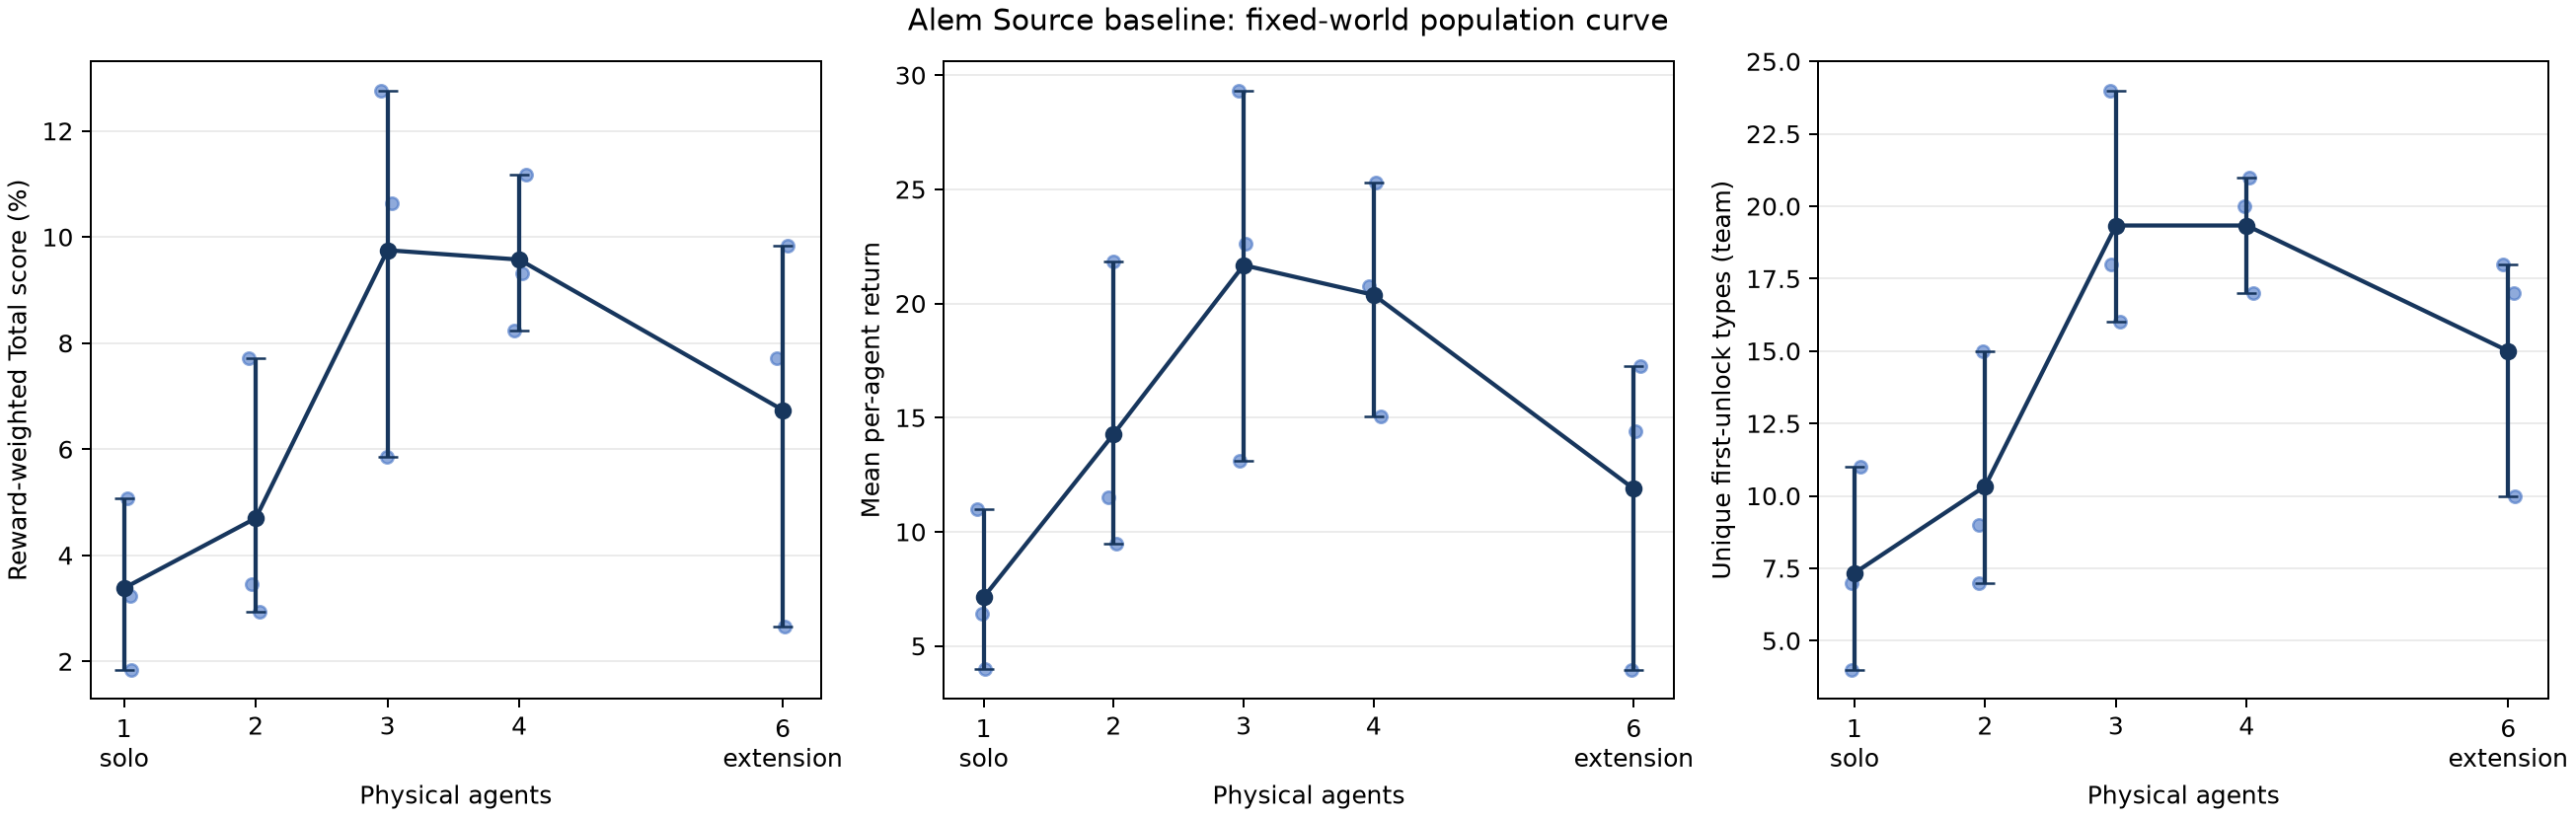
\includegraphics[width=\textwidth]{../../Results/e1_source_scaling/performance_vs_agents.png}
\caption{Completed Source fixed-world broadcast population screen.  Light
points are individual seeds; dark points and bars are seed means and
descriptive bootstrap intervals.  Population changes more than physical-agent
count, and the six-agent arm includes the feasibility defect described below.}
\label{fig:e1-source-scaling}
\end{figure}

Performance is non-monotonic.  Relative to $N=1$, mean Total score increased by
6.372 points at $N=3$ (descriptive interval $[4.008,9.540]$) and 6.195 points at
$N=4$ ($[3.176,9.327]$).  The $N=3$ and $N=4$ means were nearly flat
($-0.177$ points, $[-3.457,5.319]$), although their composition changed:
Base fell by 3.994 points while Coordination rose by 5.031.  All three paired
$N=6-N=3$ Total differences were negative; their mean was $-3.014$ points
($[-3.191,-2.926]$).  The $N=6-N=4$ mean was $-2.837$ points
($[-8.511,0.532]$), driven mainly by Coordination ($-6.080$ points) rather
than Base ($-0.461$ points).

$N=4$ and $N=6$ attained the same mean sum of per-agent first-unlocks, 42.33,
but team-unique first-unlocks fell from 19.33 to 15.00.  The additional agents
therefore repeated achievement types without broadening the team's observed
repertoire.

\subsection{Unnormalized events and execution cost}

Event families below are canonical cumulative counters but have heterogeneous
units and must not be added together.  Transfers are reported as
successes/attempts.

\begin{table}[ht]
\centering
\small
\begin{tabular}{@{}rrrrrrrr@{}}
\toprule
$N$ & Coord. attempts & Coord. successes & Rate & Transfers & Requests &
Revives & Deaths\\
\midrule
2 & 65  & 11 & 16.9\% & 12/12 & 20 & 0 & 0\\
3 & 60  & 5  & 8.3\%  & 20/20 & 33 & 0 & 4\\
4 & 85  & 11 & 12.9\% & 71/71 & 70 & 4 & 1\\
6 & 153 & 9  & 5.9\%  & 78/78 & 79 & 2 & 2\\
\bottomrule
\end{tabular}
\caption{E1 unnormalized event totals over three seeds.  Coordination is
undefined for the solo wrapper.  Simple Request/Give transfer remained
mechanically reliable; simultaneous coordination did not.}
\label{tab:e1-events}
\end{table}

Across the three $N=6$ episodes, only one of 69 recorded synchronous attempts
succeeded; the other eight coordination successes were seven handovers and one
elite-combat event.
Compared with $N=4$, $N=6$ generated 80\% more coordination attempts but
18.2\% fewer successes.

\begin{table}[ht]
\centering
\small
\resizebox{\textwidth}{!}{%
\begin{tabular}{@{}rrrrrrrr@{}}
\toprule
$N$ & Calls/episode & Total tokens/episode & Cache frac. & Tick wall (s) &
Delivered bytes/episode & Actionable frac. & Parse failures/episode\\
\midrule
1 & 200  & 0.863M & 0.000 & 4.546  & 0       & 1.000 & 0.33\\
2 & 400  & 2.593M & 0.302 & 6.899  & 19,671  & 0.958 & 2.00\\
3 & 591  & 3.877M & 0.294 & 8.661  & 66,736  & 0.869 & 5.00\\
4 & 800  & 5.591M & 0.279 & 10.329 & 148,177 & 0.941 & 11.33\\
6 & 1200 & 9.126M & 0.258 & 14.648 & 421,603 & 0.901 & 15.33\\
\bottomrule
\end{tabular}}
\caption{Mean E1 cost and execution exposure.  Calls within a tick overlap, so
summed model latency may exceed episode wall time.  Delivered bytes are
ordinary Source broadcast fan-out bytes, not provider traffic.}
\label{tab:e1-cost}
\end{table}

From $N=4$ to $N=6$, mean logical calls increased 50\%, total tokens 63.2\%,
delivered bytes 184.5\%, and complete-tick wall time 41.8\%.  Delivered bytes
per submitted turn rose from 49.2 at $N=2$ to 351.3 at $N=6$.  This is direct
evidence that unrestricted peer broadcast is not communication-bounded as the
population grows.

\subsection{Noop causes and action--communication divergence}

At $N=6$, the mean 169.33 effective Noops per episode decomposed exactly into
119.33 inactive turns, 34.67 intentional actionable waits, and 15.33 parser
fallbacks, with zero validation or unexplained residual fallback.  Inactivity
therefore explains 70.5\% of six-agent Noops.  It does not by itself explain
the score drop: the $N=6$ actionable fraction was 0.901, above the $N=3$
fraction of 0.869.

The parser failures were genuine behavior mismatches.  For example, an agent
that reasoned about chopping and announced that it was acting emitted
\code{<action><action>Do</action></action>}; the frozen Source parser correctly
failed closed to \code{Noop}.  However, seed 13102 had only seven parse
failures and still produced zero coordination successes despite 514,150
delivered bytes.  Communication volume and stated intent were therefore not
sufficient for synchronized physical execution.

\subsection{Six-agent geometric feasibility defect}

The $N=6$ decline cannot be interpreted as an intrinsic limit of decentralized
reasoning.  Source world generation samples some hard synchronous mining and
construction requirements as the full physical population.  At $N=6$, those
sites require six simultaneous targeters.  Yet \code{Do} affects only the
cardinal tile an agent faces, and movement prevents two players from occupying
the same position.  At most four collision-free agents can therefore target
one tile, making a hard six-agent mining or construction site impossible.

Seed 13102 exposed the failure mode clearly.  Agents mentioned the impossible
tree at coordinate $(22,26)$ in 182 messages across 80 distinct ticks and made
75 explicit ``all six'' or ``six-agent'' announcements.  At representative
synchronization ticks, only two agents selected \code{Do}; others moved or
waited, and some messages incorrectly treated diagonal positions as valid
targeting positions.  That seed obtained Coordination score 0, Total score
2.660, and zero coordination successes.

E1b is consequently valid as a \emph{Source-as-implemented stress
characterization}, not as a clean causal test beyond four agents.  The frozen
E3b0 comparison can isolate recruitment conditional on a shared feasibility
cap by pairing feasibility-fixed Source with recruitment under that identical
cap.  Explaining the E1 population drop additionally requires a separate
paired native-Source versus feasibility-fixed-Source ablation.  A paired $N=4$
check, where a four-agent cap changes nothing, is the negative-control
population.  Every attempted target must log its requirement, hard/soft
status, positions, facings, acting count, failure reason, and geometric
feasibility.

\subsection{E1 decision}

H1a receives descriptive support for a non-monotonic Source curve, not for
monotonic scalability.  H1b is supported: broadcast delivery cost grows much
faster than useful achievement breadth.  H1c is supported descriptively:
$N=6$ consumed materially more communication, tokens, and wall time while
performing below $N=3$--4.  The result motivates team-scoped routing, but does
not validate dynamic team formation, distributed task planning, context
management, or long-term role alignment.

\section{E2 preregistration: RecruitmentArena-6}

\subsection{Purpose and information structure}

E2 isolates recruitment before altering Alem.  RecruitmentArena is a
deterministic, pure-Python six-agent environment.  Each episode contains two
Warrior-, two Forager-, and two Miner-oriented private capability vectors and
private task-specific costs.  Public task cards contain a stable task ID,
three-dimensional demand, required team size two or three, reward, and
deadline.

The information boundary is:

\begin{itemize}
  \item an agent knows its own true capabilities and costs;
  \item all agents see public task cards and delivered recruitment records;
  \item other agents' true capabilities and costs remain private;
  \item published claims are public but need not equal private truth;
  \item true values are used only for terminal scoring, calibration, and the
  analysis-only oracle; and
  \item no oracle value enters an agent prompt or live allocation decision.
\end{itemize}

Episodes last 12 recruitment rounds.  Control records arrive after a one-round
delay.  Each agent may emit at most one recruitment-control record per round,
capped at 256 UTF-8 bytes.  Ordinary conversation is disabled before a team
locks and then delivered only to members of that task-bound team.  An agent may
belong to at most one active team.  Membership ends on completion,
cancellation, or deadline expiry.

\subsection{Scenario families}

Four paired scenario families isolate different allocation problems:

\begin{enumerate}
  \item one feasible complementary task;
  \item two disjoint tasks;
  \item competing tasks requiring a scarce capability; and
  \item oversubscription with more candidates than roster slots.
\end{enumerate}

Formation-only episodes complete a task deterministically when the locked
roster's true capabilities satisfy its card.  This separates formation quality
from embodied execution.  E2e later adds a five-round execution bridge.

\subsection{Decentralized methods and controls}

\paragraph{Open volunteer quorum.}
Agents publish applications.  Every peer derives the same first-valid roster
from the delayed public ledger.  Selected members explicitly accept before the
team locks.

\paragraph{Mutual nomination.}
Agents publish candidate rosters.  A team activates only when every listed
member has published the same reciprocal roster.

\paragraph{Peer Contract Net.}
A deterministic task sponsor is selected from ordinary embodied agents by a
stable task-ID hash.  The sponsor publishes a call for proposals, candidates
bid, the sponsor awards a roster from visible bids, and every selected member
accepts.

Controls are:

\begin{itemize}
  \item one preformed all-six communication team;
  \item balanced fixed $3+3$ teams;
  \item no team and no ordinary communication;
  \item deterministic random allocation; and
  \item an offline oracle ceiling that never enters an agent prompt.
\end{itemize}

\subsection{Versioned formation protocol}

The planned TFP1 control plane includes task announcement, application,
nomination, call for proposals, bid, award, accept, decline, lock, cancel,
complete, and lease-expiry events.  The canonical runtime must enforce:

\begin{itemize}
  \item strict parsing and canonical serialization;
  \item the 256-byte UTF-8 limit by rejection, never truncation;
  \item one team per agent;
  \item reciprocal roster agreement before lock;
  \item task-bound completion, cancellation, and expiry;
  \item one-round delivery delay;
  \item public control versus team-private ordinary routes;
  \item deterministic transition sequence numbers and replay hashes; and
  \item zero ordinary cross-team deliveries.
\end{itemize}

The runtime validates events and routes.  It must not choose an environment
action or silently repair a failed model record.

\subsection{E2a implementation amendment before canonical execution}

A provider-free diagnostic matrix exposed three design ambiguities before any
canonical E2 result was created.  We therefore froze the following
clarifications on 23 July 2026.

All task cards are active concurrently.  A locked roster remains committed
until a common allocation close after twelve acting rounds and a one-round
delivery drain.  Feasible teams are scored and completed together at that
close.  This prevents a scarce agent from being released and reused serially,
and makes the live allocation comparable to the static
\code{(tasks + idle)\textasciicircum6} oracle.

The weak Miner vector is $(20,20,35)$.  The provisional value 65 was invalid
for the intended scarcity test: with additive team coverage, a nonspecialist's
20 plus 65 already exceeds the mining demand of 80.  Only the strong Miner at
$(20,20,90)$ can now satisfy either scarce card.

Each decentralized protocol is crossed with two bounded task-choice policies:

\begin{description}[style=nextline,leftmargin=1.5em]
  \item[\code{local\_commit}.]
  Each agent selects one task from public cards using only its own capability,
  its private cost, and a stable public tie-break.  Mutual Nomination uses only
  the public role proxy because that protocol publishes no capability bid.
  Interest pools are disjoint and communication is low.
  \item[\code{public\_sweep}.]
  Every agent submits at most one bounded record per round while sweeping all
  tasks in stable order.  Candidate overlaps are resolved from the delayed
  public ledger; no private cross-agent state enters the decision.  This spends
  more control bytes to expose a larger candidate set.
\end{description}

The promotion denominator is oracle-allocation coverage: completed tasks
divided by the number simultaneously allocable by the exact oracle.
Individually feasible-card formation is reported separately; in the scarce
family both cards are individually feasible even though at most one can be
allocated.  We additionally record achieved utility, utility regret only at
equal reward, achieved and oracle raw cost, the oracle assignment,
candidate-roster overlap, multi-offer rounds, and roster revisions.

The all-six and fixed $3+3$ controls are topology references rather than exact
rosters.  Their raw reward and communication are retained, but normalized
oracle reward and regret are marked not applicable.  Fixed groups receive
tasks by public order without consulting hidden capability truth, and no group
is reused in the simultaneous allocation window.

\subsection{E2b sequential selector amendment before hosted execution}

The original E2b preregistration left a truth-free selector extension point but
set both methods to \code{selector=none}.  After that freeze, and before any
hosted E2b response, the canonical provider-free E2d2 replication completed
12,000 episodes.  Under truthful public claims,
\code{joint\_exact\_allocation} achieved complete task coverage, matched the
oracle allocation cost, and had zero utility regret in the constructed
cross-task conflict.  This result does not test strategic misreporting, model
compliance, or embodied execution.

The prospectively dated 23 July 2026 amendment therefore changes only the live
selector attached to Open Volunteer/Public Sweep:

\begin{itemize}
  \item Open Volunteer replicas compute
  \code{joint\_exact\_allocation} from public task cards, delivered
  application self-claims, and current public leases.
  \item Mutual Nomination remains its native reciprocal rule, labelled
  \code{native\_mutual\_reciprocal}, as the cost-sensitive comparator.
  \item The pure selector receives no other agent's true capability or cost,
  pending control, feasibility outcome, or oracle value.
  \item The enumeration assigns each available agent one task-or-idle label;
  every selected team therefore has the exact requested size and allocations
  are cross-task exclusive.
  \item The directory independently revalidates delivered applications,
  claimed feasibility, exact size, and public lease conflicts.  Members still
  issue delayed \code{ACCEPT} controls and the native sponsor still issues
  \code{LOCK}.
\end{itemize}

This is a sequential mechanism substitution inside the frozen two-method
matrix, not an added arm.  The three seeds, four families, 24 episodes,
12-round horizon, model settings, output grammar, canary gate, and hard caps
remain unchanged: 2,160 logical calls, 4,320 provider reservations, and
73,543,680 worst-case provider-attempt token reservations.  Focused
provider-free tests reproduce the E2d2 conflict, show invariance to truth-field
perturbations outside public claims, establish six-replica agreement, and
exercise exact exclusive plans through lock and replay.  No E2b behavioral
result is yet available.  An amended provider-free fake-client staging smoke
passed the canary gate and resumed through all 24 atomic markers, using 416
fake logical calls and 832 provider-attempt reservations; these values validate
orchestration only.

\subsection{E2b prelaunch safety amendment before hosted execution}

A second prospectively dated amendment was applied on 23 July 2026 after an
independent prelaunch review and still before any hosted E2b response.  It
changes provenance, dispatch accounting, and response-envelope validation,
but no prompt content, selector, scenario, behavioral outcome, or comparison.
Hosted launch now fails closed before output creation or client construction
unless credentials, canonical Git \code{HEAD} and status, \code{uv.lock}, all
source hashes, this protocol, and the config hash agree.  The only permitted
dirty path is the exact untracked global replay artifact, whose content hash
is recorded.

One nonblocking lock is held over the entire output root.  Before each
dispatch, a hash-chained JSONL ledger durably appends and \code{fsync}s a
reservation keyed by cell, round, agent, and semantic attempt.  A crash leaves
that reservation spent and stops automatic resume; completed-cell markers
must exactly cover all reservations and resolutions.  Cross-cell execution is
sequential by default.  Explicit \code{--parallel-cells --workers N} is safe
because cells write disjoint paths while reservation append and all three
campaign budgets are locked.  Within-round six-agent concurrency is
unchanged, and canary promotion remains sequential.

The input reservation now adds 1,024 framing tokens to the conservative
one-token-per-prompt-byte charge.  Consequently the executable cap is
77,967,360 provider-attempt tokens; the all-repair theoretical maxima are
62,373,888 recorded-success tokens and 124,747,776 provider-attempt tokens.
Actual input above prompt bytes plus framing, output above 1,024, or more than
two attempts fails closed, and provider \code{Retry-After} is clamped to 30
seconds.

For this arm only, the Responses adapter preserves the completion exactly,
including outer whitespace and CR/LF.  A valid envelope must be
\code{completed}, have no incomplete reason, have a nonempty response ID, and
return either the exact \code{gpt-5.6-luna} alias or that alias with a valid
\code{YYYY-MM-DD} snapshot suffix.  The resolved model is stable in the
canary and exact-bound throughout the full stage.  Marker schema v2
recomputes prompt bytes, raw hashes, the strict 256-byte TFP1 parse, normalized
records, call/token counts, reservations, replay state and audit chains,
deterministic hashes, and terminal analysis.  The stored canary gate must be
canonically identical to a pure recomputation over the one expected cell, and
every gate predicate must be true.

Provider-free regressions cover crash reservations, concurrent-lock
exclusion, ledger and marker tampering, copied cells, changed derived
analysis, wrong or dated-invalid models, incomplete responses, missing IDs,
raw whitespace/newlines, 256/257-byte boundaries, usage overages, and retry
clamping.  A post-hardening fake canary-to-full lifecycle used three explicit
cell workers and completed all 24 markers with 416 logical calls, 832 provider
reservations, 4,213,422 framing-aware token reservations, no unresolved
reservation, and no overage.  The first attempt exposed an overly global
mid-run unresolved check; the corrected validator scopes that check to the
cell while the final campaign gate remains global, and a regression pins this
behavior.  These checks establish orchestration integrity only; no E2b
behavioral evidence has yet been collected.

\subsection{E2b adversarial recovery amendment before hosted execution}

A third prospectively dated amendment was applied on 23 July 2026 after a
second independent adversarial review and before any hosted or network-backed
E2b response.  It changes no prompt, role, selector, seed, scenario, horizon,
outcome, or cap.  It closes five recovery paths by advancing the campaign,
protocol/config, prompt-cache, and default output identities to v3 and the
anchored reservation ledger to v2.

First, E2b now explicitly requests a strict Responses envelope.  Missing model
identity, missing usage, and missing or non-exact
\code{input\_tokens}/\code{output\_tokens} fail before a call record can be
accepted.  Booleans, strings, floats, and nulls are never coerced.  A present
cache or reasoning counter is subject to the same exact-integer rule, while an
omitted optional detail remains zero.  The strict switch defaults off in the
shared adapter, independently of exact completion preservation, so ordinary
adapter behavior is unchanged.  A malformed envelope consequently cannot
write a comprehensively valid cell or promotion gate.

Second, reservation ledger v2 couples every reservation and resolution record
to a separately created, exclusive, \code{fsync}ed hash-chain anchor.  Each
manifest checkpoint binds record count, canonical ledger-prefix hash,
record-chain head, anchor count, and anchor-chain head.  The 18 logical calls
of a complete canary therefore produce 36 anchored events; truncating a
valid suffix while leaving the durable anchor high-water is a hard failure,
not a fresh 18-call budget.  Existing files are also fail-closed: a partial
artifact triple, a complete but invalid triple, an unexpected managed file,
or any cell file beside an empty ledger cannot be classified as pending.

Third, the managed root must be both lexical-canonical and realpath-contained.
Managed opens use \code{O\_NOFOLLOW}, regular-file checks, and link count one.
Symlinked components and artifact directories, parent/root aliases,
hardlinked locks, ledgers or artifacts, and two separately locked roots that
share an artifact are rejected.  Creation durably synchronizes every newly
created ancestor, the directory itself, and its parent.

Finally, any provider-usage overage or reservation-resolution integrity
failure permanently poisons the campaign.  No new reservation may dispatch;
queued cell futures are cancelled when possible, whereas an already in-flight
request may only complete its durable resolution.  The final bound manifest
records the poison and reason.  A failed or poisoned manifest cannot be
resumed to reset that state, and ledger overages or unresolved reservations
independently stop recovery.

The focused offline adversarial suite exercises exact usage and model
identity, malformed-envelope non-promotion, valid-prefix canary truncation,
partial/invalid/empty-ledger artifacts, path aliases and cross-root sharing,
ancestor durability, sticky poison, in-flight resolution, resolution callback
failure, and poisoned resume.  A fresh fake-client lifecycle passed canary,
then completed all 24 cells with three explicit cell workers: 464 logical
calls, 928 provider-attempt reservations, 4,694,278 reserved tokens, 928
ledger events and 928 anchors, with zero unresolved reservations, zero
overages, and no poison.  Repeating full resume constructed no provider client
and preserved the exact 928-event checkpoint.  These measurements validate
only offline orchestration and recovery.  They provide no evidence yet about
Luna recruitment behavior or comparative efficacy.

\subsection{E2b v2 hosted failure and prospective v3 amendment}

The first bounded hosted attempt was launched from commit
\hash{345da487a0217776b89b655e693dadcbfb153807} into the explicit v2 root.
Its Open Volunteer/single-complementary canary passed all then-current gates.
The promoted three-worker stage subsequently failed and poisoned itself:
the full manifest contains 3 completed-marker entries, 2 failed Mutual cells,
and 19 cancelled cells after 72 logical calls, 144 provider reservations, and
706,642 reserved tokens.  This is a failed diagnostic, not an incomplete
method comparison.  The root is preserved and cannot resume.

The read-only summarizer binds this evidence in
\path{Results/e2b_v2_failed_diagnostic_v1.json} and its Markdown rendering.
The root-tree, full-manifest, and ledger SHA-256 values are, respectively,
\hash{406b4f09c1d5ae8e532bfaee0c9aa591324eb0603f0063635b54997c1ed374e0},
\hash{14c90f60f5348472f00421842e552d623b282fa1a13ad08b4563d8a72d84fbd0},
and
\hash{950f5a7ce4ec3386bba2853e6409a5310496e5d5c69bc061a59e96cf3bcd4f04}.
It classifies only the original 18-call Open/single canary as an eligible
partial diagnostic.  Open/two-disjoint made 22 calls and reached 0.5
oracle-allocation coverage, but it also records 12 poison-budget abstentions
and is explicitly excluded.  A zero-call poison artifact, both failed Mutual
cells, and all cancelled cells are likewise excluded; no value is imputed.

The archived call envelopes identify a concrete output-budget failure.  Nine
of 72 calls returned \code{incomplete/max\_output\_tokens}; every one used
exactly 1,024 output tokens, all 1,024 were reasoning tokens, and the visible
completion was blank.  The single and two-disjoint Mutual cells contained
four and five such calls, respectively.  Two other Mutual outputs were
well-formed nominations that omitted their own sender from the roster and
failed \code{semantic.sender\_missing}.  Thus the evidence supports an
output-censoring diagnosis and records a separate coordination error, but
does not support a comparative efficacy claim.

Because completed responses already reached 1,020 output tokens, the
right-censored sample cannot establish that 2,048 would clear the
high-reasoning tail.  Before any v3 response, the successor therefore freezes
4,096 output tokens.  This is four times the censoring boundary, while the
input-dominated per-attempt reservation grows only 17.0\%, from 18,048 to
21,120 tokens.  The visible TFP1 grammar remains capped at 256 bytes.  Any
v3 max-output truncation is still invalid; the cap is never adapted after a
v3 observation.

V3 also replaces the one-method canary with four seed-22000 cells: both Open
Volunteer and Mutual Nomination crossed with single-complementary and
two-disjoint.  Each cell must independently pass replay, envelope, transport,
invalid-call, repair, budget, and no-truncation gates and form at least one
truly feasible team.  All requested/resolved model bindings must agree.  A
missing, failed, invalid, poison-affected, zero-call, or nonforming cell blocks
full-stage client construction.

The full logical/provider limits remain 2,160 and 4,320; the 4,096-token
output allowance raises the hard provider-attempt exposure to 91,238,400.
The four-cell canary projects at most 360 logical calls, 720 provider
reservations, and 15,206,400 reserved tokens under the 25\% repair gate.  A
fresh offline fake lifecycle passed all four canary cells and completed 24/24
full cells with three workers: 440 logical calls, 880 provider reservations,
7,157,450 reserved tokens, 880 ledger events/anchors, no unresolved
reservation, no overage, and no poison.  A repeat full resume constructed no
client and changed no checkpoint.  At that amendment freeze, no hosted v3
call had been made.

\subsection{E2b v3 negative Mutual screen and Open-only v4 protocol}

V3 was subsequently launched from commit
\hash{ddcbb92fb0ff0376216bf0aa3da84e246945bad7} into the explicit v3 root.
Its four-cell canary failed after 40 logical calls, 80 provider-attempt
reservations, and 614,968 reserved tokens.  The manifest contains one
completed Open cell, two failed cells, and one cancelled cell; the shared
budget is poisoned and the root cannot resume.

The deterministic read-only evidence is stored in
\path{Results/e2b_v3_failed_diagnostic_v1.json} and its Markdown rendering.
The root-tree, canary-manifest, and ledger SHA-256 values are, respectively,
\hash{d88e134f203f11363aadbce502bf9c9b22682c660046465870477c887fb70899},
\hash{fd565c10968300d81ec60876ecf6a6cf0ba4556b3934abda0b97e6c06f84baad},
and
\hash{f4275aeec46bb2a2338cf9f5b3ad7ea36b4fc1499787eb3817804bfac6bc77e6}.
The report classifies Open/single as the sole eligible partial diagnostic,
Mutual/single as a failed mechanism diagnostic, Open/two as a zero-call
poison cascade, and Mutual/two as cancelled.  No cell is imputed.

The larger generation allowance removed the v2 censoring failure: all 40 v3
calls completed, with zero max-output truncation and zero transport error.
Open/single again formed a truly feasible team, locking roster $[0,5]$ for
full coverage and reward 100 in 18 calls.  The Open/two worker made no model
call because another cell had already poisoned the shared campaign; its 12
budget abstentions do not measure Open behavior.

Mutual/single gives a negative screen of the frozen mechanism.  Its 22 calls
all completed, but five nominations omitted their own sender.  Sender 2
nominated \code{MEMBERS=0,1}, and its semantic repair repeated the identical
invalid record; sender 3 produced the same roster.  Senders 5 and 1 each
nominated \code{MEMBERS=0,2} while omitting themselves.  The cell nevertheless
locked $[0,2]$, which was truly infeasible, yielding zero oracle-allocation
coverage and zero reward.  Together with the v2 sender-omission signal, this
supports stopping the frozen Mutual arm rather than repeatedly tuning its
prompt.  A self-inclusion instruction or specialized repair would define a
new exploratory mechanism, not a correction inside the confirmatory result.

Before any v4 response, v4 was prospectively frozen as Open Volunteer with the
truth-free joint exact allocator, retaining the model, high reasoning,
4,096-token allowance,
TFP1 grammar, seeds, families, and 12-round horizon.  Its 12 episodes are
$3$ seeds $\times$ $4$ families $\times$ one method.  A fresh campaign-v4
identity and output root prevent either failed predecessor from resuming.
The seed-22000 canary contains Open/single and Open/two; both must pass every
integrity, model-binding, rate, no-truncation, and true-feasible-formation
gate before the remaining ten cells may run in parallel.

The two-cell canary projects at most 180 logical calls, 360 provider
reservations, and 7,603,200 reserved tokens.  Full v4 caps are 1,080 logical
calls, 2,160 provider reservations, and 45,619,200 reserved tokens.  A
provider-free lifecycle passed both canary cells, completed 12/12 cells with
three workers, and resumed without constructing a client.  It used 272
logical calls, 544 provider reservations, 4,555,934 reserved tokens, and 544
ledger records/anchors, with no unresolved reservation, overage, or poison.
At the protocol freeze this validated orchestration only; no hosted v4 call
had yet been made.

\subsection{E2b v4 completed hosted result}

The hosted campaign was subsequently launched from clean source commit
\hash{2092ebcb3e059f57acaed8e2b56460ec2b69ab8d} into the explicit v4 root.
The immutable root-tree, canary-manifest, canary-gate, full-manifest, and
reservation-ledger SHA-256 values are, respectively,
\hash{36ba9a6445293896fec943f0145b075520a6f524136d8324e8a8e162957c221c},
\hash{0560637ee7e75aa3992450dfe82eac9d0fbb44649a917590c4f71f3d84a46cc4},
\hash{d1ae8b56f9032d93043f102efa5566f47dab5c446442cbebe43d8bce645015c1},
\hash{d263c7aecbc032cc117b1084c9eac246e3b04ac614592befa949d4664b50ad02},
and
\hash{6096f58d2496d0b9fa0062dce9e4aa31adc9971179e7f5e13366e26f9759cb4f}.
The deterministic read-only evidence is stored in
\path{Results/e2b_v4_hosted_results_v1.json} and its Markdown rendering.
Before deriving results, the summarizer reuses the launcher's strict
artifact, debug-shard, directory-replay, checkpoint, and durable-ledger
validators.  All 12 cells and 586 anchored ledger records validated, covering
293 unique reservations and resolutions with no unresolved reservation,
overage, poison, failed episode, or cancellation.

\begin{table}[ht]
\centering
\small
\resizebox{\textwidth}{!}{%
\begin{tabular}{@{}lrrrrrrrr@{}}
\toprule
Partition & Cells & Full reward & Full coverage & Calls & Repairs & Invalid &
Input tokens & Output tokens\\
\midrule
Canary, separate & 2 & 2/2 & 2/2 & 36 & 0 & 0 & 29,874 & 7,504\\
Promoted invocation, new cells & 10 & 10/10 & 10/10 & 257 & 2 & 2 &
232,091 & 70,285\\
Combined evidence & 12 & 12/12 & 12/12 & 293 & 2 & 2 &
261,965 & 77,789\\
\bottomrule
\end{tabular}}
\caption{E2b v4 stage accounting.  The promoted full manifest is cumulative:
it began with the two bound canary cells and dispatched only the other ten
using three cell workers.  Canary and promoted invocation wall times were
24.412 and 89.432 seconds, respectively.}
\label{tab:e2b-v4-stage}
\end{table}

Every family passed all three seeds.  Across the 12 episodes, all 15 locked
teams were truly feasible and no true-infeasible team locked.  Ten complete
task-to-roster allocations exactly equalled the true-information oracle;
12 of 15 individual task rosters matched.  Table~\ref{tab:e2b-v4-family}
therefore reports allocation quality in addition to reward.

\begin{table}[ht]
\centering
\small
\begin{tabular}{@{}lrrrrrr@{}}
\toprule
Family & Cells & Calls & Mean rounds & Exact alloc. & Utility regret & Cost delta\\
\midrule
Single complementary & 3 & 54 & 4.000 & 3/3 & 0.000000 & 0.000\\
Oversubscribed & 3 & 54 & 4.000 & 2/3 & 0.003889 & 4.667\\
Scarce capability & 3 & 99 & 6.667 & 3/3 & 0.000000 & 0.000\\
Two disjoint & 3 & 86 & 6.000 & 2/3 & 0.018750 & 15.000\\
\midrule
All & 12 & 293 & 5.167 & 10/12 & 0.005660 & 4.917\\
\bottomrule
\end{tabular}
\caption{E2b v4 hosted outcomes.  Regret and cost use true generated profiles
and are descriptive means over three seeds per family.}
\label{tab:e2b-v4-family}
\end{table}

The two non-oracle allocations retained full feasibility and reward but
committed using the public bids available before every later useful bid was
present.  Oversubscribed seed 22001 incurred $+14$ raw cost.  Two-disjoint
seed 22002 incurred $+45$ and did not lock its second team until round 8.
This is an observed two-cell association, not a causal estimate; it motivates
a separately frozen bid-closure/quorum or provisional-lock-grace ablation.

The 293 logical calls comprise 291 initial decisions and two semantic repairs;
all used one provider attempt.  There were zero transport errors, incomplete
responses, or max-output truncations.  Actual usage was 261,965 input plus
77,789 output tokens, including 72,168 reasoning tokens.  Mean and maximum
call latency were 3.281 and 12.004 seconds; summed round-decision wall time was
281.622 seconds.  The two invalid initial decisions (0.687\%) were an
\code{ACCEPT} before its roster was ready and an already-teamed agent applying
to a second task.  Both repairs returned a valid abstention.

The agents emitted 133 valid control submissions.  The replay recorded 127
accepted and six rejected delivered transitions, 6,340 payload bytes, and
30,410 delivered bytes, or 2,534.2 per episode.  Seventy-five of 76 submitted
capability vectors and all 76 costs exactly matched the private profile.  The
one mismatch reported $[0,80,20]$ instead of $[20,80,20]$; the omitted
nondemanded component did not alter feasibility or reward, but prevents a
perfect profile-reporting claim.

Provider-free E2d2's scripted truthful joint-exact arm provides context: it
achieved full reward/coverage with zero regret/cost delta over 4,000 episodes.
It used different seeds, Contract-Net behavior, and phase timing, so its
values are not a paired causal baseline for hosted v4.

V4 passes the mechanism screen and promotes only Open Volunteer/Public Sweep
with truth-free joint exact allocation to a bounded, paired E3 Alem transfer
with Source action behavior unchanged.  It does not establish Open superiority
over a redesigned Mutual method, embodied task efficacy, population
scalability, or long-horizon role alignment.

\subsection{Member-selection ablation}

Holding Peer Contract Net fixed, E2d compares:

\begin{enumerate}
  \item \code{first\_valid}: first claimed-feasible roster by arrival round and
  agent ID;
  \item \code{random\_valid}: deterministic seeded sampling from
  claimed-feasible rosters; and
  \item \code{exact\_utility}: exact enumeration of subsets of the required
  size.
\end{enumerate}

For claimed capability vector $q_i$, cost $c_{it}$, and task demand $d_t$,
the exact rule maximizes
\[
U(S,t)=
\min_{j:d_{tj}>0}
\frac{\sum_{i\in S}q_{ij}}{d_{tj}}
-
0.25\frac{\sum_{i\in S}c_{it}}{100|S|}.
\]
A roster is claimed-feasible only if it has the requested size and coverage of
at least one in every demanded dimension.  Utility ties resolve by
lexicographically sorted agent IDs.  The analysis-only oracle enumerates
\((\text{tasks}+\text{idle})^6\) assignments using true capabilities and costs.

\subsection{E2 stages and hypotheses}

\begin{table}[ht]
\centering
\small
\begin{tabular}{@{}llll@{}}
\toprule
Stage & Seeds & Model use & Purpose\\
\midrule
E2a & 20000--20999 & None & Scripted correctness and determinism\\
E2b & 22000--22002 & GPT-5.6 Luna high & LLM mechanism screen\\
E2c & 22100--22109 & GPT-5.4 nano high & Paired efficacy estimate\\
E2d & 22200--22209 & Fixed contract net & Selection-rule ablation\\
E2e & 22300--22309 & GPT-5.4 nano high & Five-round execution bridge\\
\bottomrule
\end{tabular}
\caption{E2 funnel.  Only methods passing the mechanism gate enter E2c.}
\label{tab:e2-design}
\end{table}

\begin{description}[style=nextline,leftmargin=1.5em]
  \item[H2a: formation.]
  At least one decentralized method will form feasible teams before deadline
  in at least 80\% of feasible opportunities.
  \item[H2b: structure.]
  Contract Net will reduce conflicting rosters relative to open volunteer
  formation, at the cost of additional control latency.
  \item[H2c: selection.]
  Exact utility will reduce oracle regret relative to first-valid and random
  selection when scarce capabilities create competing feasible rosters.
  \item[H2d: communication boundary.]
  Team-private execution will use fewer delivered ordinary-message bytes than
  all-six communication while maintaining complementary completion.
\end{description}

Primary E2 outcomes are normalized task reward and oracle regret.  Secondary
outcomes are formation latency, feasible-team rate, churn, roster agreement,
truthful-report calibration, messages, delivered bytes, tokens, and wall time.

\plannedfigure{Paired normalized reward and oracle regret by recruitment method,
followed by formation latency and delivered-byte efficiency.}

\plannedresult{Record E2a as an engineering result before any paid call.  For
E2b--E2e, preserve raw model output and rejection codes; do not rewrite invalid
messages.  If no method passes the mechanism gate, stop before E3, version the
protocol, and preserve the negative result.}

\section{E3 preregistration: recruitment in Alem}

\subsection{Treatment semantics}

E3 introduces recruitment only through opt-in topologies.  The baseline
topology remains behaviorally unchanged.

\begin{itemize}
  \item An unteamed agent may emit only one valid bounded TFP1 record on the
  public bulletin.
  \item Invalid, oversized, or free-form unteamed messages are rejected,
  logged, and delivered to no one.
  \item Once a roster locks, ordinary Source-style
  \code{<communication>} text is delivered only to current teammates.
  \item Nonmembers receive no ordinary team-message copy.
  \item Public control traffic and private ordinary traffic are charged and
  reported separately.
  \item Membership changes take effect deterministically after the accepted
  lock transition and are replayable from the event journal.
  \item Middleware validates and routes; it does not select an Alem action.
\end{itemize}

This is a team-scoped \emph{communication} study, not strict information
isolation.  Ordinary Alem teammate observations remain visible.  Environment
Requests and targeted \code{Give} are not filtered by team in the initial E3
study.

\subsection{Observable tasks and stable identity}

An embodied agent must locally observe an opportunity before announcing it.
Stable task IDs derive only from observable task type, dungeon level, and
location.  The current text wrapper is insufficient by itself because it
collapses multiple same-type coordination cues and normally omits absolute
coordinates.  E3 therefore requires structured, locally visible opportunity
metadata generated from the same light and view masks as the agent's text.
This metadata may validate and identify an agent-selected announcement; it
must not trigger an automatic announcement or expose a hidden opportunity.

Before E3a, the task taxonomy and capability mapping must be frozen for
coordinated mining, construction, elite combat, and handover opportunities.
All arms in the first E3 study use the 48-by-48 world and task requirements of
two or three agents.

\subsection{Critical environment control}

At six agents, current world generation sometimes assigns the full physical
population as the requirement for mining, construction, and elite-mob
coordination.  Although an environment field named
\code{max\_agents\_required} exists, current generation does not apply it.
For mining and construction, a six-agent hard requirement is geometrically
unsatisfiable: non-overlapping players can target a single tile only from its
four cardinal neighbors.  Changing this globally would silently alter the
Source scaling environment and erase the native defect measured by E1.

The E3 implementation must therefore add an explicit, experiment-only
two-to-three-agent requirement control.  It must be enabled identically for
every E3 comparison arm and disabled by default so E0/E1 world generation is
unchanged.  The generator consumes the same random draws and then clamps a
full-population hard-mining outcome to three; existing two-agent outcomes
remain two-agent outcomes.  The controlled Source arm is unchanged in policy,
prompt, parser, timing, and route, but it is not a reuse of the native E1
$N=6$ environment.

\subsection{Frozen narrow transfer protocol and current gate}

The first transfer is frozen separately as protocol
\code{alem-dice-e3b0-open-joint-hard-mining-v1}.  It narrows the broader E3
program to hard synchronous mining and compares only:

\begin{enumerate}
  \item six-agent Source broadcast in the shared feasibility-controlled world;
  and
  \item the identical one-call-per-agent action path with Open Volunteer,
  replicated truth-free joint exact allocation, and team-scoped ordinary
  routing.
\end{enumerate}

There is no leader, commander, planner, second action call, or hidden-state
selector.  The public control plane is strict TFP1; invalid unteamed free text
fails closed without changing the agent's environment action.  At most two
public task cards may be active.  Cards require teams of two or three, use
one-tick-delayed public records, and close deterministically on completion,
expiry, cancellation, or coordinate disappearance.

This protocol is prospective and not runnable at the present checkpoint.
Provider-free E3a must first prove unchanged Source prompt/action/route bytes,
zero unauthorized ordinary deliveries, deterministic directory replay,
receiver-specific byte accounting, public-selector replica agreement, local
task provenance, stale-record rejection, and safe release of every lease.
Only after every E3a predicate passes may E3b0 issue its single provider
preflight and paired three-seed, 200-tick screen.  The E3b0 outcome cannot
explain the native E1 defect; a separate native-versus-feasibility-fixed Source
ablation is required for that question.

\subsection{Arms, stages, and hypotheses}

E3 compares:

\begin{enumerate}
  \item unchanged six-agent Source full broadcast;
  \item balanced fixed $3+3$ communication teams;
  \item dynamic recruitment using the promoted E2 method and selection rule;
  \item a bulletin-only, no-ordinary-conversation screening floor.
\end{enumerate}

The final paper-scale comparison retains Source, fixed $3+3$, and dynamic
recruitment.  A second recruitment method is retained only if its normalized
reward is within 5\% of the best method while materially reducing
communication.

\begin{table}[ht]
\centering
\small
\begin{tabular}{@{}lllll@{}}
\toprule
Stage & Environment & Seeds & Horizon & Purpose\\
\midrule
E3a & Alem Debug, scripted god mode & 14000--14001 & 20 & Route correctness\\
E3b & Alem Debug, Easy & 14100--14102 & 200 & Paid mechanism screen\\
E3c & Full Alem, Easy & 14200--14209 & 1,000 & Paired efficacy estimate\\
E3d & Full Alem, all difficulties & 14300--14319 & 10,000 & Paper scale\\
\bottomrule
\end{tabular}
\caption{E3 funnel.  E3d requires explicit cost authorization.}
\label{tab:e3-design}
\end{table}

\begin{description}[style=nextline,leftmargin=1.5em]
  \item[H3a: transfer.]
  A mechanism passing E2 will form valid task teams under Alem's observation
  and survival constraints.
  \item[H3b: communication efficiency.]
  Dynamic recruitment will reduce ordinary delivered bytes relative to
  all-six Source broadcast.
  \item[H3c: performance preservation.]
  The communication reduction will not reduce any co-primary outcome by more
  than the preregistered 5\% relative margin in the final paired comparison.
  \item[H3d: adaptivity.]
  Dynamic teams will outperform fixed $3+3$ teams on scenarios where task
  locations and capability needs change during the episode.
\end{description}

\plannedfigure{Performance--communication frontier for Source broadcast, fixed
$3+3$, dynamic recruitment, and the bulletin-only floor.}

\plannedresult{E3 results may be added only after E3a demonstrates zero
unauthorized ordinary deliveries, deterministic membership replay, and
unchanged baseline prompts/routes.  Report locally observed task provenance and
every rejected control record.}

\section{Promotion rules and statistical reporting}

\subsection{Mechanism gates}

Every implemented recruitment mechanism must satisfy:

\begin{itemize}
  \item zero unauthorized cross-team ordinary deliveries;
  \item 100\% roster agreement for every activated team;
  \item at least 95\% action and recruitment-transition validity;
  \item zero unrecovered provider failures in canonical episodes;
  \item at least 80\% of feasible opportunities formed before deadline;
  \item matching deterministic replay hashes; and
  \item no baseline prompt or route change under baseline topology.
\end{itemize}

These are eligibility gates, not outcomes that may be averaged away.  A routing
violation blocks efficacy interpretation even if reward is high.

\subsection{Behavioral promotion}

For a ten-seed behavioral promotion, a treatment must have positive paired
direction on at least seven of ten seeds for at least two of Total percentage,
mean per-agent return, and unique team achievements, with no material
regression in the third.  Effect sizes and paired uncertainty are reported even
when this directional rule fails.

A final communication-efficiency claim requires a paired 95\% interval showing
no worse than a 5\% relative performance margin on all three co-primary
outcomes while reducing delivered communication bytes by at least 30\%.
Communication cost and model-token cost are reported separately.

\subsection{Multiple views of cost}

Every behavioral table includes:

\begin{itemize}
  \item total model calls and calls per actual agent-tick;
  \item input, output, reasoning, cache-read, and cache-write tokens;
  \item emitted payload bytes and fan-out-weighted delivered bytes;
  \item control-plane and ordinary-message bytes separately;
  \item summed model latency and complete tick wall time; and
  \item requested versus executed ticks and alive-agent-step exposure.
\end{itemize}

The coordination-efficiency diagnostic is
\[
\text{coordination efficiency}=
\frac{\text{paired team-performance improvement}}
     {\text{delivered communication bytes}},
\]
reported alongside its numerator and denominator rather than as a standalone
ranking.

\section{Implementation readiness and risk register}

E2 now has a deterministic TFP1 runtime, RecruitmentArena, selectors,
analysis-only oracle, provider-free tests, and a staged resumable E2b launcher.
Its fake-client canary-to-full smoke validates orchestration and accounting,
not behavior.  E3-specific Alem task extraction and opt-in receiver-specific
routing remain absent.  The evaluator supplies parallel calls, one-tick
broadcast, route accounting, and canonical artifacts, while E0 supplies
six-agent compatibility evidence.  The older DCP1 parser remains distinct from
TFP1 and must not be used as evidence for task cards, membership, leases, byte
caps, or receiver-specific routing.

\begin{longtable}{@{}p{0.18\textwidth}p{0.27\textwidth}p{0.47\textwidth}@{}}
\caption{Pre-implementation E2/E3 risk register.}
\label{tab:risks}\\
\toprule
Risk & Failure mode & Required mitigation\\
\midrule
\endfirsthead
\toprule
Risk & Failure mode & Required mitigation\\
\midrule
\endhead
Baseline route drift &
A routing refactor changes Source delivery, order, delay, or accounting. &
Keep the existing baseline branch explicit; add golden prompt and
$N(N-1)$ route regressions before dynamic routing.\\
\addlinespace
Global task-size change &
Applying a three-agent cap globally changes E1's $N=4/6$ worlds. &
Use an opt-in E3-only requirement control, identical across E3 arms and disabled
by default.\\
\addlinespace
Unstable task IDs &
Text cues omit absolute location or collapse multiple opportunities. &
Expose structured locally visible opportunities from the same visibility mask;
never inspect or announce hidden tasks.\\
\addlinespace
Byte-limit corruption &
Truncation turns one invalid record into a different apparent record. &
Measure the complete UTF-8 payload and reject records above 256 bytes.\\
\addlinespace
Hidden allocation &
Middleware or oracle chooses a roster or action using private truth. &
Use only published claims for live selection; reserve true values for scoring
and the offline oracle.\\
\addlinespace
Roster disagreement &
Agents act on different membership states after delayed messages. &
Require reciprocal acceptance, canonical transition order, per-agent ledger
comparison, and deterministic replay.\\
\addlinespace
Cross-team leakage &
One sender-indexed broadcast map delivers private text to all agents. &
Use receiver-indexed delivery envelopes for opt-in team topologies and assert
zero nonmember recipients.\\
\addlinespace
Protocol noncompliance &
LLM output is malformed, oversized, stale, or unauthorized. &
Log stable rejection codes, deliver nothing, and never silently rewrite a live
record.\\
\addlinespace
Prompt confound &
Recruitment instructions accidentally alter the baseline condition. &
Inject formation context only under explicit recruitment/fixed-team settings;
snapshot baseline prompts.\\
\addlinespace
Premature efficacy claim &
Reward is analyzed despite mechanism or replay failure. &
Apply structural promotion gates first and preserve stopped/negative studies.\\
\addlinespace
Cost confound &
Different episode-worker concurrency changes provider load by arm. &
Use one episode worker, concurrent within-tick agents, randomized sequential
blocks, and complete usage accounting.\\
\bottomrule
\end{longtable}

\section{Audit and provenance requirements}

Every canonical study records:

\begin{itemize}
  \item resolved configuration and exact CLI invocation;
  \item Git commit, branch, dirty-source manifest, dependency lock/hash, Python
  version, and platform;
  \item model snapshot, reasoning effort, cache policy, and nominal call ceiling;
  \item scenario or environment seeds and paired-arm mapping;
  \item raw prompts, raw responses, provider response IDs, finish reasons,
  usage, retries, and transport errors;
  \item parsed actions and recruitment events with stable validation codes;
  \item task cards, event sequence, roster transitions, leases, route envelopes,
  rejected deliveries, and replay hashes;
  \item terminal metrics and actual agent-tick denominators; and
  \item the exact CSV/JSON inputs for every table and figure.
\end{itemize}

Artifacts from failed or partial attempts are archived rather than overwritten.
Canonical episodes require terminal status and no API/runtime error.
Resumption retries only failed seeds.  Paid stages begin with a dry-run
call/token ceiling and a clean committed implementation.

\subsection{Completed E0 provenance}

E0 ran from
\path{2026-07-23T06:24:16.409143Z} to
\path{2026-07-23T06:28:23.047401Z} at commit
\hash{587e7176ce3b02296120e9504c1d7d609e9dcf2a}.  Its raw root is
\path{outputs/alem_eval/e0_agent_compatibility_v1}.  The source-of-truth result
SHA-256 is
\hash{7b67b56544a00df63b1e07106c9eeffe51eedc9bc62dc7d8d914af734ad8c47d}.

\subsection{Completed E0.1 provenance}

The complete E0.1 matrix ran from
\path{2026-07-23T06:57:25.963656Z} to
\path{2026-07-23T07:08:25.236294Z} using measured-run commit
\hash{5c4c64338b9aae9132f9cc32b6eec3d746964529}.  Its raw root is
\path{outputs/alem_eval/e0_1_agent_compatibility_200_v2}.  The source-of-truth
result SHA-256 is
\hash{6d28e885e241b4f58553291d6fa205fb982878f2575f6bdd3a24d711fda9b529}.
The earlier diagnostic attempt remains at
\path{outputs/alem_eval/e0_1_agent_compatibility_200_v1}; it stopped after the
two $N=1$ episodes under the original strict validator.

\subsection{Completed E1 provenance}

E1 measured the trusted Source tree at
\hash{49bc152e2b70609aa9a4518b86b1f8f1fced5a14}.  Its canonical raw root is
\path{outputs/alem_eval/e1_source_scaling_3seed_200_v2}; the study-manifest
SHA-256 is
\hash{fc1ae646345f644fc645ce8f09aa005c259cef23d76844f9bbdf9c6dfe642b7e}.
The corrected analyzer and generated evidence were committed through
\hash{af1417d2029772ba0d5bc351d6b25ddc6b84c7dd}.  The committed summary JSON,
episode CSV, and paired-contrast CSV SHA-256 values are, respectively,
\hash{3818cf6ecdde3be7ce9c8daf16a04ad5ad759cac402ff53212a4051b68fc0e10},
\hash{2d4a2a25ada4b1cde918a24facf8baf08e3bfbc1ea24dd77d231b7507d084388},
and
\hash{92768988e054bcdf3ff37931a33557962438c68e1a2f04a87ee9fbc4e29d36a5}.
The strict replay reconstructed all 91 episode columns, 300 population
estimates, 600 paired estimates, 4,219 ordinary communication routes, and all
token, latency, retry, and ledger totals from the raw evidence.

The E0/E0.1 source manifests recorded the pre-existing untracked replay
\path{Results/replays/nano_high_source_full_world.mp4}.  It was outside the run
roots and was not an input to either result.

\section{Interpretation rules and limitations}

\begin{itemize}
  \item E0 and E0.1 establish engineering compatibility only.  Their
  \code{Noop} returns and mortality are not behavioral scaling evidence.
  \item E1 is a descriptive fixed-world population curve.  It cannot isolate
  agent count from role balance, spawn geometry, prompt growth, mob pressure,
  or coordination requirements.
  \item $N=1$ uses a different solo wrapper.  $N=6$ is beyond the paper's
  documented one-to-four range and can generate hard six-agent mining or
  construction requirements that cannot be satisfied from the four
  collision-free cardinal target positions.  Its regression is therefore not
  evidence that adding agents intrinsically harms coordination.
  \item E2's formation-only reward is a mechanism diagnostic, not evidence that
  a team can navigate or execute in Alem.  E2e and E3 address that gap.
  \item E2b v2 is a failed, method-incomplete campaign.  Its one eligible Open
  canary and excluded poison-affected artifacts cannot estimate an Open-versus-
  Mutual effect.  V3 eliminated truncation in 40 calls but produced only one
  uncontaminated Open cell and one failed Mutual cell, so it supports a
  negative mechanism screen rather than a comparative effect.  Open-only v4
  passed its own mechanism gate, but it still cannot establish that Open is
  superior to a repaired or redesigned Mutual mechanism.
  \item V4 has only three seeds per family in a structured formation arena.
  Its 12/12 reward/coverage outcome warrants bounded environment transfer, not
  an embodied-efficacy, population-scaling, or long-horizon role-alignment
  claim.  The two non-oracle allocations also show that full reward is
  insufficient evidence of optimal team assignment.
  \item E2b's rollback defense creates and synchronizes one anchor for every
  reservation and resolution: two anchor files per logical provider call.
  This does not add model calls or tokens, but it adds local metadata and
  \code{fsync} latency.  Hosted v4 created 586 anchors for 293 calls.  The
  canary and promoted invocations took 24.412 and 89.432 seconds, but the
  design does not separately identify local durability overhead from provider
  and scheduling latency.
  \item E3 isolates ordinary message routing, not all channels of information
  or resource transfer.
  \item High reward cannot validate a method that leaks messages, disagrees on
  rosters, or uses hidden information.
  \item A result from three seeds is a mechanism screen, not confirmatory
  efficacy evidence.  Ten- and twenty-seed stages retain raw paired effects and
  uncertainty.
  \item E3d and other 10,000-tick paid stages require explicit authorization
  after a fresh estimate.
\end{itemize}

\section{Planned final synthesis}

The final report will answer the research questions in causal order:

\begin{enumerate}
  \item Does unchanged Source behavior improve, plateau, or degrade as $N$
  increases, and at what communication/token cost?
  \item Which decentralized recruitment protocol most reliably forms feasible
  teams under the bounded bulletin?
  \item Does mathematically informed selection reduce oracle regret?
  \item Does the promoted mechanism preserve performance when execution and
  survival are restored?
  \item Does team-scoped communication reduce delivered bytes without exceeding
  the 5\% performance-regression margin?
\end{enumerate}

\begin{table}[ht]
\centering
\small
\begin{tabularx}{\textwidth}{@{}X l X@{}}
\toprule
Claim & Status & Evidence boundary\\
\midrule
The evaluator supports variable physical populations. & \pass &
E0/E0.1 structural, accounting, replay, and renderer gates.\\
Source-as-implemented performance is non-monotonic over $N=1,2,3,4,6$. &
\pass{} descriptive & E1, three paired seeds and coarse uncertainty.\\
The native $N=6$ drop is caused by agent-count scaling. & \fail{} unsupported &
Hard six-agent targets can be geometrically impossible; causal feasibility
ablation pending.\\
Open Volunteer plus public joint allocation can form bounded synthetic teams. &
\pass{} screen & E2b v4, 12/12 cells and 15/15 true-feasible locks.\\
Open is superior to other decentralized recruitment methods. &
\fail{} unsupported & V4 had no live comparator; Mutual v2/v3 was a failed
frozen mechanism, not a fair effect estimate.\\
Team-scoped formation improves embodied Alem execution. & \pending &
E3a routing/task gates and E3b0 paired action-loop screen unrun.\\
Context management preserves long-horizon role alignment. & \pending &
No completed stage measures this abstract claim.\\
\bottomrule
\end{tabularx}
\caption{Current claim-by-evidence ledger.  A failed unsupported claim is a
boundary on interpretation, not necessarily evidence of the opposite.}
\label{tab:claim-ledger}
\end{table}

\section{Current conclusion}

Alem's canonical language-agent evaluation path supports one, two, three,
four, and six physical agents under the tested provider-free conditions.  E0
passed its short compatibility gate.  E0.1 passed every structural gate but
failed the literal full-horizon requirement because three inactive-policy
episodes ended naturally.

E1 now supplies the first behavioral population screen.  Source performance
improved through three agents and remained similar at four, while six agents
used substantially more tokens, communication, and wall time without
increasing achievement breadth.  That result is useful systems evidence but
not a clean intrinsic scaling law: native six-agent worlds can contain hard
synchronous targets that are geometrically unsatisfiable.

E2 now supplies both a bounded negative and a bounded positive mechanism
result.  Raising the output allowance removed the observed v2 truncation, but
frozen Mutual Nomination still produced repeated self-omission and a
true-infeasible lock in v3.  The separately frozen Open-only v4 screen then
formed 15/15 true-feasible teams and achieved full reward/coverage in all 12
cells with two repaired semantic errors and no provider failure.  However,
only 10/12 allocations exactly matched the oracle, and one capability claim
was inexact.  The evidence therefore promotes Open Volunteer with joint exact
allocation only to a bounded paired Alem transfer; it does not establish Open
superiority, embodied coordination efficacy, population-scale improvement, or
long-horizon role coherence.

The immediate next stage is provider-free E3a, not another paid efficacy run.
It must implement and prove opt-in task provenance, deterministic Open
Volunteer state, replicated truth-free allocation, team-only ordinary routes,
unchanged Source bytes, and a shared experiment-only feasibility control.  A
paid E3b0 screen is eligible only if those gates pass.  The native-versus-fixed
Source ablation remains separately necessary before interpreting the E1
six-agent regression.  Downstream claims must continue to be updated from
canonical artifacts rather than console summaries.

\appendix

\section{Reproduction commands for completed gates}

\paragraph{E0.}
\begin{quote}
\small\ttfamily\raggedright
uv run --extra baselines-llm --python 3.12 \textbackslash\\
\quad python scripts/run\_e0\_agent\_compatibility.py \textbackslash\\
\quad --output outputs/alem\_eval/e0\_agent\_compatibility\_v1
\end{quote}

\paragraph{E0.1.}
\begin{quote}
\small\ttfamily\raggedright
uv run --extra baselines-llm --python 3.12 \textbackslash\\
\quad python scripts/run\_e0\_agent\_compatibility.py \textbackslash\\
\quad --counts 1,2,3,4,6 \textbackslash\\
\quad --seeds 13000,13001 \textbackslash\\
\quad --steps 200 \textbackslash\\
\quad --output
outputs/alem\_eval/e0\_1\_agent\_compatibility\_200\_v2
\end{quote}

\paragraph{E1 strict Source population summary (zero provider calls).}
\begin{quote}
\small\ttfamily\raggedright
uv run --extra baselines-llm --python 3.12 \textbackslash\\
\quad python scripts/summarize\_source\_scaling\_e1.py \textbackslash\\
\quad outputs/alem\_eval/e1\_source\_scaling\_3seed\_200\_v2
\textbackslash\\
\quad --bootstrap-reps 10000 --bootstrap-seed 8675309 \textbackslash\\
\quad --out Results/e1\_source\_scaling
\end{quote}

\paragraph{E2b v4 deterministic hosted-result summary (zero provider calls).}
\begin{quote}
\small\ttfamily\raggedright
uv run --extra baselines-llm --python 3.12 \textbackslash\\
\quad python scripts/summarize\_recruitment\_llm\_success.py \textbackslash\\
\quad /home/adam/Desktop/AlemDICE/outputs/recruitment\_llm/
e2b\_luna\_screen\_v4 \textbackslash\\
\quad --json-output Results/e2b\_v4\_hosted\_results\_v1.json
\textbackslash\\
\quad --markdown-output Results/e2b\_v4\_hosted\_results\_v1.md
\end{quote}

\section{Result-table inventory}

\begin{enumerate}
  \item Completed E1 population-by-seed co-primary outcomes and cost metrics.
  \item Completed E1 paired bootstrap intervals and population trend contrasts.
  \item E2a scenario-by-method mechanism gates.
  \item E2b/c raw validity, formation, reward, regret, and cost.
  \item E2d roster-selection utility and oracle-regret contrasts.
  \item E2e formation-to-execution attrition and team-private delivery audit.
  \item E3a route-invariant and task-provenance audit.
  \item E3b/c paired Source, fixed-team, and dynamic-team outcomes.
  \item E3 performance--communication noninferiority analysis.
  \item Final claim-by-evidence and negative-result table.
\end{enumerate}

\section{Deferred extensions}

Strict filtering of teammate observations, Requests, and \code{Give};
message loss; crash-stop and Byzantine agents; reputation learning; teams
larger than three; populations above six; learned routing; and long-horizon
context or role-drift studies are outside E0--E3.  They require separate
protocols rather than post-hoc interpretation of this program.

\end{document}
